% mobi.tex:

\chapter{MODULAR OPTICAL BRAIN IMAGER (MOBI)} % all caps please
\label{chap:mobi}


\section{Introduction} %significance
\label{chap:mobi:introduction}
Neuroimaging techniques have advanced our fundamental understanding of human brain function~\cite{Crum2021}. However, brain activations often exhibit complex patterns and dynamics that are only apparent when measured in natural environments~\cite{Park2018, Crum2021}. Despite making tremendous progress, contemporary neuroimaging techniques such as \ac{fMRI}~\cite{Heinzel2013} and \ac{MEG} are hindered from studying these advanced dynamics due to their poor portability and immobility during use~\cite{Herold2017, Yucel2017}. \ac{EEG}, although highly portable, suffers from low spatial resolution compared to \ac{fMRI}~\cite{Sirpal2019, Herold2017}. These inherent disadvantages of the gold standard techniques restrict our current understanding to limited types of stimuli and interactions within confined spaces~\cite{Park2018}. In recent years, researchers have turned to \ac{fNIRS} to address this technological gap~\cite{Boas2014}. FNIRS is based on the theory of neurovascular coupling~\cite{Ferrari2012}. It uses low-power light spectroscopy to measure brain activation and its associated hemodynamics~\cite{Boas2014}. With its non-invasive nature, the use of \ac{fNIRS} has increased exponentially~\cite{Quaresima2019, Yucel2017} to include studies from psychiatric conditions~\cite{Ehlis2014, Kumar2017} and language~\cite{Quaresima2012, Rossi2012, Jackson2019} to cognitive neurodevelopment~\cite{Aslin2015, Vanderwert2014, Wilcox2015, Soltanlou2018} and stroke recovery~\cite{Yang2019}, education~\cite{Brockington2018}, pain detection~\cite{LopezMartinez2019}, and even brain-computer interfaces~\cite{Naseer2015, Ahn2017, Hong2018}.

Many of these studies using \ac{fNIRS} have utilized traditional, fiber-based, cart-sized instrumentation~\cite{Scholkmann2014, Eggebrecht2014, Wheelock2019, Everdell2005}. Despite it being an improvement over conventional \ac{fMRI} and \ac{MEG} modalities, fiber-based \ac{fNIRS} systems also quickly reached a limit on portability and channel density due to the use of fragile fiber optic cables~\cite{Saikia2019, Zhao2019} and stationary source/detector units~\cite{Oxymon2017, Techen2018}. The need to expand toward broader paradigms in unrestricted environments~\cite{Crum2021} requires the use of portable and wearable systems~\cite{Curtin2018, Park2018}, and the need for wearable systems has led to the increased use of modular architectures~\cite{Bci2017, Zimmermann2013, Funane2017, Wyser2017, Zhao2020, VidalRosas2021, Liu2022}. 

Modular \ac{fNIRS} systems are probes composed of repeating source/detector circuits called modules~\cite{Chitnis2016}. Repeating modules not only facilitate and lower fabrication costs but also allow for reconfigurability to varying sizes of regions of interest~\cite{Zhao2017}. By using only the minimal number of modules needed for a specific task, modular \ac{fNIRS} systems drastically improve portability~\cite{Yucel2017}. Additionally, the use of varying \ac{SD} separations by utilizing both intra- and inter-module (sources and detectors on different modules) pairs provide overlapping channels, improving both spatial resolution and depth specificity (a key parameter in removing systemic physiological signals)~\cite{Gregg2010, VidalRosas2021}. Modern \ac{fNIRS} systems now leverage a plethora of state-of-the-art design and analysis tools that support the use of modular architecture in natural environments. Optode layout optimizers~\cite{Machado2018, Aasted2015, ZimeoMorais2018, Brigadoi2018} and modular probe designers~\cite{Vanegas2022} ensure application-specific arrangements, motion~\cite{Huppert2009, Santosa2018} and coupling~\cite{Hernandez2020} artifact correction algorithms allow for improvements in data quality, and faster light-propagation simulation tools~\cite{Nirfast,Fang2009} facilitate the use and analysis of high-density \ac{fNIRS} probes. 

Despite its increasing adoption, the modular high-density \ac{fNIRS} architecture also possesses its own set of technical challenges~\cite{Pinti2018, Herold2017} and usability concerns~\cite{Moon2019, Hasan2022}. First, the use of \ac{fNIRS} in natural settings means subjects will be more mobile, leading to headgear moving and shifting relative to the scalp during use~\cite{Herold2017, Perrey2014}. Current solutions to ensure proper coupling use mechanical components that are cumbersome, require replacements, and add head-borne weight~\cite{Bartkowski2019, Bci2017}. Second, the ever-increasing number of optodes in a probe requires very efficient encoding strategies to maintain sufficiently high frame rates to capture the hemodynamic response function~\cite{Maki1995, Everdell2005, Alper2022}. Finally, in order to improve accuracy using high-density tomographic analysis, we must be able to know the location of all optodes in a probe prior to and during the use of a system~\cite{Mazzonetto2022}. The most traditional approach is to use expensive hand-held 3-D digitizing systems to record the coordinates of optodes prior to the start of an experiment~\cite{Pinti2018, Zhao2020}. More recent solutions leveraging photogrammetry promise to be more portable, but still require a set of external cameras that restrict mobility to areas within the camera's field of view~\cite{VidalRosas2021, Mazzonetto2022}. 

To address these needs, we have designed a lightweight and re-configurable \ac{fNIRS} Modular Optical Brain Imager (\ac{MOBI}) system well-suited for full-head long-term brain monitoring or over a particular \ac{ROI}. This ultra-compact and fiberless system addresses optode-to-scalp contact coupling through its shape and board composition. A dual-triangle shape allows for better conforming to a surface, akin to how a triangular mesh accurately represents a 3-D shape, while its flexible-circuit-based board allows the entire module to bend over arbitrary shapes to ensure constant optode-to-scalp contact~\cite{Bartkowski2019, Muehlemann2008}. Additionally, a dense \ac{P2P} network allows the system to automatically determine the connection topology between modules of a probe without user input. This facilitates the implementation of a spatial multiplexing encoding strategy to increase a probe's full frame rate. Finally, the wearable \ac{MOBI} modules each contain 3-D orientation sensors that leverage the connection topology and the module's geometry to automatically determine the location of all sources and detectors without the use of an external hand-held or photogrammetry tracking system. This automatic, independent digitization method shortens setup times, ensures high data quality, and improves accuracy and contrast through tomographic reconstructions.

In this paper, we introduce our \ac{MOBI} system. In Section~\ref{chap:mobi:methods}, we describe our entire \ac{MOBI} system design, including details of individual modules as well as supporting components such as the master and trigger boards. We also highlight novel features of our system, including connection topology recognition, IMU-based optode positioning, and frame rate improvement through spatial multiplexing. Section~\ref{chap:mobi:results} focuses on the characterization of our \ac{MOBI} module and the validation of its features. We quantify conformability through the use of flexible-circuit-based modules and detail the accuracy of our internal-based optode digitization method. Additionally, we show results from two \emph{in-vivo} experiments and compare \ac{MOBI}'s performance to that of a commercial \ac{fNIRS} system. Finally, Section~\ref{chap:mobi:discussion} describes the limitations and assumptions used in our investigation and proposes work to address them in the future.  




%%%% METHODS %%%%
\section{Methods}
\label{chap:mobi:methods}

\subsection{Module design}
\begin{figure}
    \centering
    \begin{minipage}{.38\textwidth}
        \begin{center}
	        \subfigure[]{\label{fig:module_top}\includegraphics[width=\linewidth]{fig/mobi/module_top.png}}
	    \end{center}
    \end{minipage}%
    \begin{minipage}{.10\textwidth}
    \end{minipage}%
    \begin{minipage}{.35\textwidth}
        \begin{center}
	        \subfigure[]{\label{fig:module_guides}\includegraphics[width=\linewidth]{fig/mobi/module_guides.png}}
	        \subfigure[]{\label{fig:module_flex}\includegraphics[width=\linewidth]{fig/mobi/module_flex.png}}
	    \end{center}  
    \end{minipage}%
	\caption{(a) Top side of a Modular Optical Brain Imager (MOBI) module without a silicone cover showing the four FPC connectors and 5 hair removal holes. (b) Bottom side of a MOBI module with light guides on optodes and black silicone cover of board. (c) Unpopulated flexible-circuit-board for a MOBI module.} 
	\label{fig:module}
\end{figure}

Our \ac{MOBI} system is based on double-sided modules manufactured on flexible-circuit-based boards, allowing the modules to bend and conform to the scalp [Fig.~\ref{fig:module_flex}]. Each module houses two detectors (OPT101, Texas Instruments, USA) with built-in trans-impedance amplifiers. The 3 dual-wavelength sources (SMT735D/850D, Marubeni, Japan) at 735 and 850~nm are driven from a digital multiplexer (NX3L4051, NXP Semiconductors, Netherlands) with a programmable constant current driver (LT3092, Analog Devices Inc., USA) using a spatial multiplexing encoding strategy (Fig.~\ref{fig:architecture_mobi}). 

The optode layout results in one 8~mm, one 30~mm, and four 24.5~mm dual-wavelength channels on a single module. A 3~mm diameter light guide (53-833, Edmund Optics, USA) is glued to each optode to focus the emitted and detected light [Fig.~\ref{fig:module_guides}]. A 9-axis inertial measurement unit (IMU) allows for absolute orientation measurements for each module (BNO055, Bosch Sensortec, Germany). All optodes and sensors on the \ac{MOBI} module are controlled and read by an onboard system-on-a-chip (BC832, Fanstel Corp, USA) with an integrated microcontroller (nRF52832, Nordic Semiconductor, Norway). An internal Inter-Integrated Circuit (I$^2$C) communication protocol is used to set the current driver and communicate with the onboard IMU (Fig.~\ref{fig:architecture_mobi}). Additionally, three low-dropout (LDO) voltage regulators regulate the power source voltage for the source, detector, and auxiliary measurement components. The microcontroller samples all six dual-wavelength channels, dark measurements, and IMU measurements at a frame rate of 22~Hz. 

\begin{figure}
	\begin{center}
	    \includegraphics[width=\textwidth]{fig/mobi/architecture_mobi.pdf}
	    %https://miro.com/app/board/uXjVPNOzApc=/
	\end{center}
	\caption{Schematic diagram of a single Modular Optical Brain Imager module. The microcontroller uses an internal Inter-Integrated Circuit (I$^2$C) protocol to communicate with components on a single board. A peer-to-peer network allows communication between neighboring modules. } 
	\label{fig:architecture_mobi}
\end{figure} 

The five optodes are located on one side of the module\textemdash the side that remains in contact with the scalp. All driving electronics are placed on the non-scalp side of the module to assist with heat dissipation and comfort. Triangles are the most efficient shape for tessellating a 3-D surface, thus, the use of a ``dual-triangle'' shape (two equilateral triangles with 50~mm sides) and a flexible-circuit-based board allows for increased conformity and optode-scalp coupling. \ac{MOBI} modules have a channel density of 0.56 dual-wavelength channels per square centimeter. The modules are completely encapsulated in flexible black silicone to provide comfort during long-term wear, block stray light, and protect the electronic components during use. Each module has four flexible printed circuit (FPC) connectors that allow multiple modules to be connected using FPC cables of fixed lengths [Fig.~\ref{fig:module_top}]. A \ac{P2P} serial network allows each module to communicate with up to four connected neighboring modules. Five 6~mm diameter holes next to each optode are used for hair removal after placement on the scalp. Each module, including the components, light guides, and silicone cover, weighs 14~grams. 

\subsection{System architecture}
\begin{figure}
	\begin{center}
        \subfigure[]{\label{fig:architecture_master}\includegraphics[width=0.8\textwidth]{fig/mobi/architecture_master.pdf}}
        %https://miro.com/app/board/uXjVPNOzApc=/
        \subfigure[]{\label{fig:master_module}\includegraphics[width=0.4\textwidth]{fig/mobi/master_module.png}}
	\end{center}
	\caption{(a) Schematic diagram of a Modular Optical Brain Imager system. An external power source and trigger board are optional. (b) The master module without its cover.} 
	\label{fig:architecture}
\end{figure} 

Our \ac{MOBI} system consists of a computer, a single master module, and an arbitrary number of \ac{MOBI} modules connected to each other using FPC cables (Fig.~\ref{fig:architecture}). Optionally, a separate power source and a trigger board can also be connected to the master module to allow synchronization of events during experiments. The master module uses an I$^2$C communication protocol for power and data acquisition of each module (Fig.~\ref{fig:architecture_master}). The master module incorporates a USB-based microcontroller development system (Teensy 4.0, PJRC, USA), a voltage regulator, an FPC connector, a Japan Solderless Terminal (JST) connector, and two switches. A micro-USB cable connects the master board to a computer for serial communication. The switches are used to manually select the power source (from micro-USB or an external battery). A 2-pin JST connector allows an external trigger board to be connected for synchronizing auxiliary signals such as experimental triggers. The trigger board is based on a simple microcontroller (Atmega328p, Microchip, USA) and interrupts \ac{fNIRS} readings from inputted Transistor-Transistor Logic (TTL) signals. The entire trigger board is encased inside a 3-D printer cover. A graphical user interface (GUI) provides real-time detector and IMU readings. The GUI also provides the ability to change the current source and detector gain of individual optodes. All acquired \ac{MOBI} data is saved in the SNIRF~\cite{snirf2021} format. 

\subsection{Automatic features}
\begin{figure}
    \begin{center}
       \subfigure[]{\label{fig:auto_demo}\includegraphics[width=.8\textwidth]{fig/mobi/auto_demo.png}}
       \subfigure[]{\label{fig:auto_gui_connection}\includegraphics[width=.3\textwidth]{fig/mobi/auto_gui_connection.png}}
       \subfigure[]{\label{fig:auto_gui_imu}\includegraphics[width=.3\textwidth]{fig/mobi/auto_gui_imu.png}}
    \end{center}
    \caption{(a) Five modules in a single chain configuration connected to a master module. (b) Modular Optical Brain Imager (MOBI) Graphical User Interface (GUI) displays 5 modules connected. (c) MOBI GUI displays the relative position of each module based on differences in neighboring IMU measurements.} 
    \label{fig:automatic}
\end{figure} 
\subsubsection{Connection topology recognition}
Our \ac{MOBI} system has the ability to recognize the connection topology between all modules to determine the number of modules and the orientation of each module in an arbitrary probe. Any two modules can be connected by simply bridging any FPC connections with an FPC cable [Fig.~\ref{fig:auto_demo}]. Upon start-up, each module samples all four of its \ac{P2P} communication channels to determine if another module is connected to one or more of its FPC connectors. This sampling of inputs/outputs allows the \ac{P2P} serial network to automatically determine how each module is laid out relative to others. With the \ac{P2P} connections identified, the master board can determine the orientation of each module in the probe by simply rotating and translating the module dimensions based on the connection topology [Fig.~\ref{fig:auto_gui_connection}]. 

\subsubsection{IMU-based optode positioning}
Additionally, our \ac{MOBI} system can automatically determine the 3-D position of each source and detector in the probe without the use of an external digitizer. With the connection topology known, the master module can sample the orientation sensors between neighboring modules to create a 3-D spline estimating the shape onto which the probe is placed [Fig.~\ref{fig:auto_gui_imu}]. The master module then superimposes FPC cable lengths, module geometry, and optode layout within a module to derive the 3-D location of each optode, reducing the need for time-consuming 3-D position measurements. The IMU measurements also permit robust temporal signal rejection through real-time monitoring of optode movements during use. 

\subsubsection{Spatial multiplexing groupings}
Finally, our \ac{MOBI} modules utilize a spatial multiplexing encoding strategy in which sources are grouped into spatial multiplexing groups (SMG) and turned on at the same time~\cite{Vanegas2022}. Based on the layout of all the sources and detectors (automatically derived from the connection topology), the master module assigns sources into SMGs to be on simultaneously without cross-talk based on the signal-to-noise ratio (SNR) of the system. In this way, probe layouts that are more spread apart lead to a smaller number of SMGs because the sources are more dispersed. The spatial multiplexing improvement ratio (IR) is defined as the number of sources in a probe divided by the number of SMGs. In this way, spatial multiplexing improves a system's full frame rate by a factor of IR. 

\subsection{In-vivo protocols}
The \ac{MOBI} system was validated against a commercial fiber-based \ac{fNIRS} system (Brite23, Artinis) through simultaneous measurements during a dual-pressure cuff occlusion experiment on the arm. A single \ac{MOBI} module and an Artinis probe with a single channel were placed on the underside of the forearm for the cuff occlusion experiment. The upper arm rested at the same height as the heart. Data from the 30~mm channels were simultaneously captured at 10~Hz in a completely dark room. The 100~mmHg (venous) and 220~mmHg (arterial) occlusions lasted 75 seconds each. 

Additionally, human brain activity was measured in an adult male in the left motor cortex area during a finger-tapping task. The finger-tapping task consisted of a 10-second task period followed by 20 seconds of rest, repeated 10 times with 60 seconds of baseline rest prior to and at the end of the repeated tasks. Subjects were instructed to sit still with their eyes closed during the entire experiment. During the task period, a verbal command instructed the subjects to tap their right thumb sequentially against their index, middle, ring, and pinky finger, followed by the same sequence mirrored, repeated as fast as possible until instructed to rest. During rest, subjects were instructed to place both hands on their laps. Signals were obtained through a single \ac{MOBI} module placed over the left motor cortex. 

Data from \ac{MOBI} were converted to SNIRF format using MOCA. Data from Artinis was first converted to the NIRS format using the Artinis software, OxySoft, prior to converting to SNIRF format using Homer. Optical density was converted to hemoglobin concentrations using Homer after applying a 0.01~Hz high-pass (HPF) and a 0.5~Hz low-pass filter (LPF) to all channels. 



%%%%%% RESULTS %%%%%%
\section{Results}
\label{chap:mobi:results}
\subsection{System characterization}
A 20-module full-head \ac{MOBI} probe results in 372 dual-wavelength channels due to the use of source and detector pairs in between adjacent modules. This increases the achievable channel density to 1.72 channels per square centimeter. Additionally, with \ac{MOBI}'s spatial multiplexing encoding strategy and a \ac{SD} separation cutoff of 52~mm (where SNR is $>$ 40~dB), this full-head probe results in 14 spatial multiplexing groups and a full frame rate of 4.7~Hz. Each source is driven at 100~mA. The total power draw of the full-head probe is 2.31~W, resulting in a 2.85-hour battery life when a 3.7~V 2000 milliamp-hour (mAh) battery is used.

%SNR + NEP + Dynamic Range
\begin{figure}
	\begin{center}
	    {\includegraphics[width=.45\textwidth]{fig/mobi/snr.pdf}}
	\end{center}
	\caption{Signal-to-noise (SNR) of Modular Optical Brain Imager modules as source-detector separation increases. Red asterisks indicate SNR for the 735~nm while black diamonds are for the 850~nm wavelength. Orange numbers signify the channel number. Channels 1, 2, and 3 are from the same module. Channels 4, 5, and 6 are from sources and detectors on different modules.} 
	\label{fig:snr}
\end{figure} 
Fig.~\ref{fig:snr} shows the signal-to-noise ratio (SNR) as a function of SD separations. The SD separations were calculated from intra- and inter-module channels using a 3-module probe placed on an optical phantom ($\mu_{s}^{'} = 4.7~cm^{-1}$ and $\mu_{a} = 0.063~cm^{-1}$ at 830~nm). Each measurement is the average of 10 samples of that channel. Fig.~\ref{fig:snr} shows a linearly decreasing SNR as SD separation increases for both wavelengths. The correlation coefficient, $R^2$, is 0.955 and 0.959 for the 735 and 850~nm wavelengths, respectively. SNR for \ac{MOBI} modules is greater than 50~dB for SD separations of up to 43~mm. 


\subsection{Spatial multiplexing improvement}
%\afterpage{%    % defer execution until the next page break occurs anyway
    \begin{figure}%[t!] % not "pt"
    	\begin{center}
     
    	   \subfigure[]{\label{fig:layout1}\includegraphics[width=.3\textwidth]{fig/mobi/layout1.pdf}}
    	   \subfigure[]{\label{fig:layout2}\includegraphics[width=.3\textwidth]{fig/mobi/layout2.pdf}}
    	   \subfigure[]{\label{fig:layout3}\includegraphics[width=.3\textwidth]{fig/mobi/layout3.pdf}}
           %\subfigure[]{\label{fig:domesetup}\includegraphics[width=.3\textwidth]{domesetup.pdf}}
    	\end{center}
    	\caption{Three example probe layouts all composed from five identical Modular Optical Brain Imager modules. Optodes are represented by small red circles (sources) and blue crosses (detectors). Each layout has multiple spatial multiplexing groups determined based on the global proximity of sources to each other. Red dashed circles show which sources are simultaneously on for the first spatial multiplexing group of each layout.} 
    	\label{fig:layouts}
    \end{figure} 
    
    \begin{table}% not t or b or p
        \centering
        \caption{The full frame rate of a probe depends on the layout of the modules within a probe. The three layouts in Figure~\ref{fig:layouts} result in the channels, groupings, and full frame rates below.}
        \label{tab:layouts}
        \begin{tabular}{lccc}
        \hline
        \multicolumn{1}{r}{}                       & Layout 1 & Layout 2 & Layout 3 \\ \hline
        Number of Modules                          & 5        & 5        & 5        \\
        Temporal Encoding Full Frame Rate {[}Hz{]} & 4.4      & 4.4      & 4.4      \\
        Number of Channels                         & 38       & 53       & 55       \\
        Number of Spatial Multiplexing Groups      & 6        & 7        & 8        \\
        Improvement Ratio                          & 2.5      & 2.14     & 1.875    \\
        Spatial Encoding Full Frame Rate {[}Hz{]}  & 11       & 9.4      & 8.25     \\ \hline
        \end{tabular}
    \end{table}
%} % end of argument of `\afterpage` command
The performance results from three different 5-module probe layouts (Fig.~\ref{fig:layouts}) are shown in Table~\ref{tab:layouts}. When using a temporal encoding strategy, the full frame rate of the probe is determined by the number of sources in the probe since each source is sampled sequentially. Although the temporal encoding full frame rate remains constant at 4.4~Hz, the channel density and the number of spatial multiplexing groups increase from layout 1 to 3 as the layout of the probe becomes denser (Row 3, Table~\ref{tab:layouts}). Consequently, the improvement ratio decreases as the probe layout increases in density, limiting the potential full frame rate performance gain. Layout 1 saw the biggest improvements in full frame rate when converting from a temporal to a spatial encoding strategy. The spatial multiplexing full frame rate was always larger than the temporal encoding full frame rate for all three layouts.  


\subsection{Optode-scalp coupling}
\begin{figure}
	\begin{center}
        \subfigure[]{\label{fig:rigid_coupling}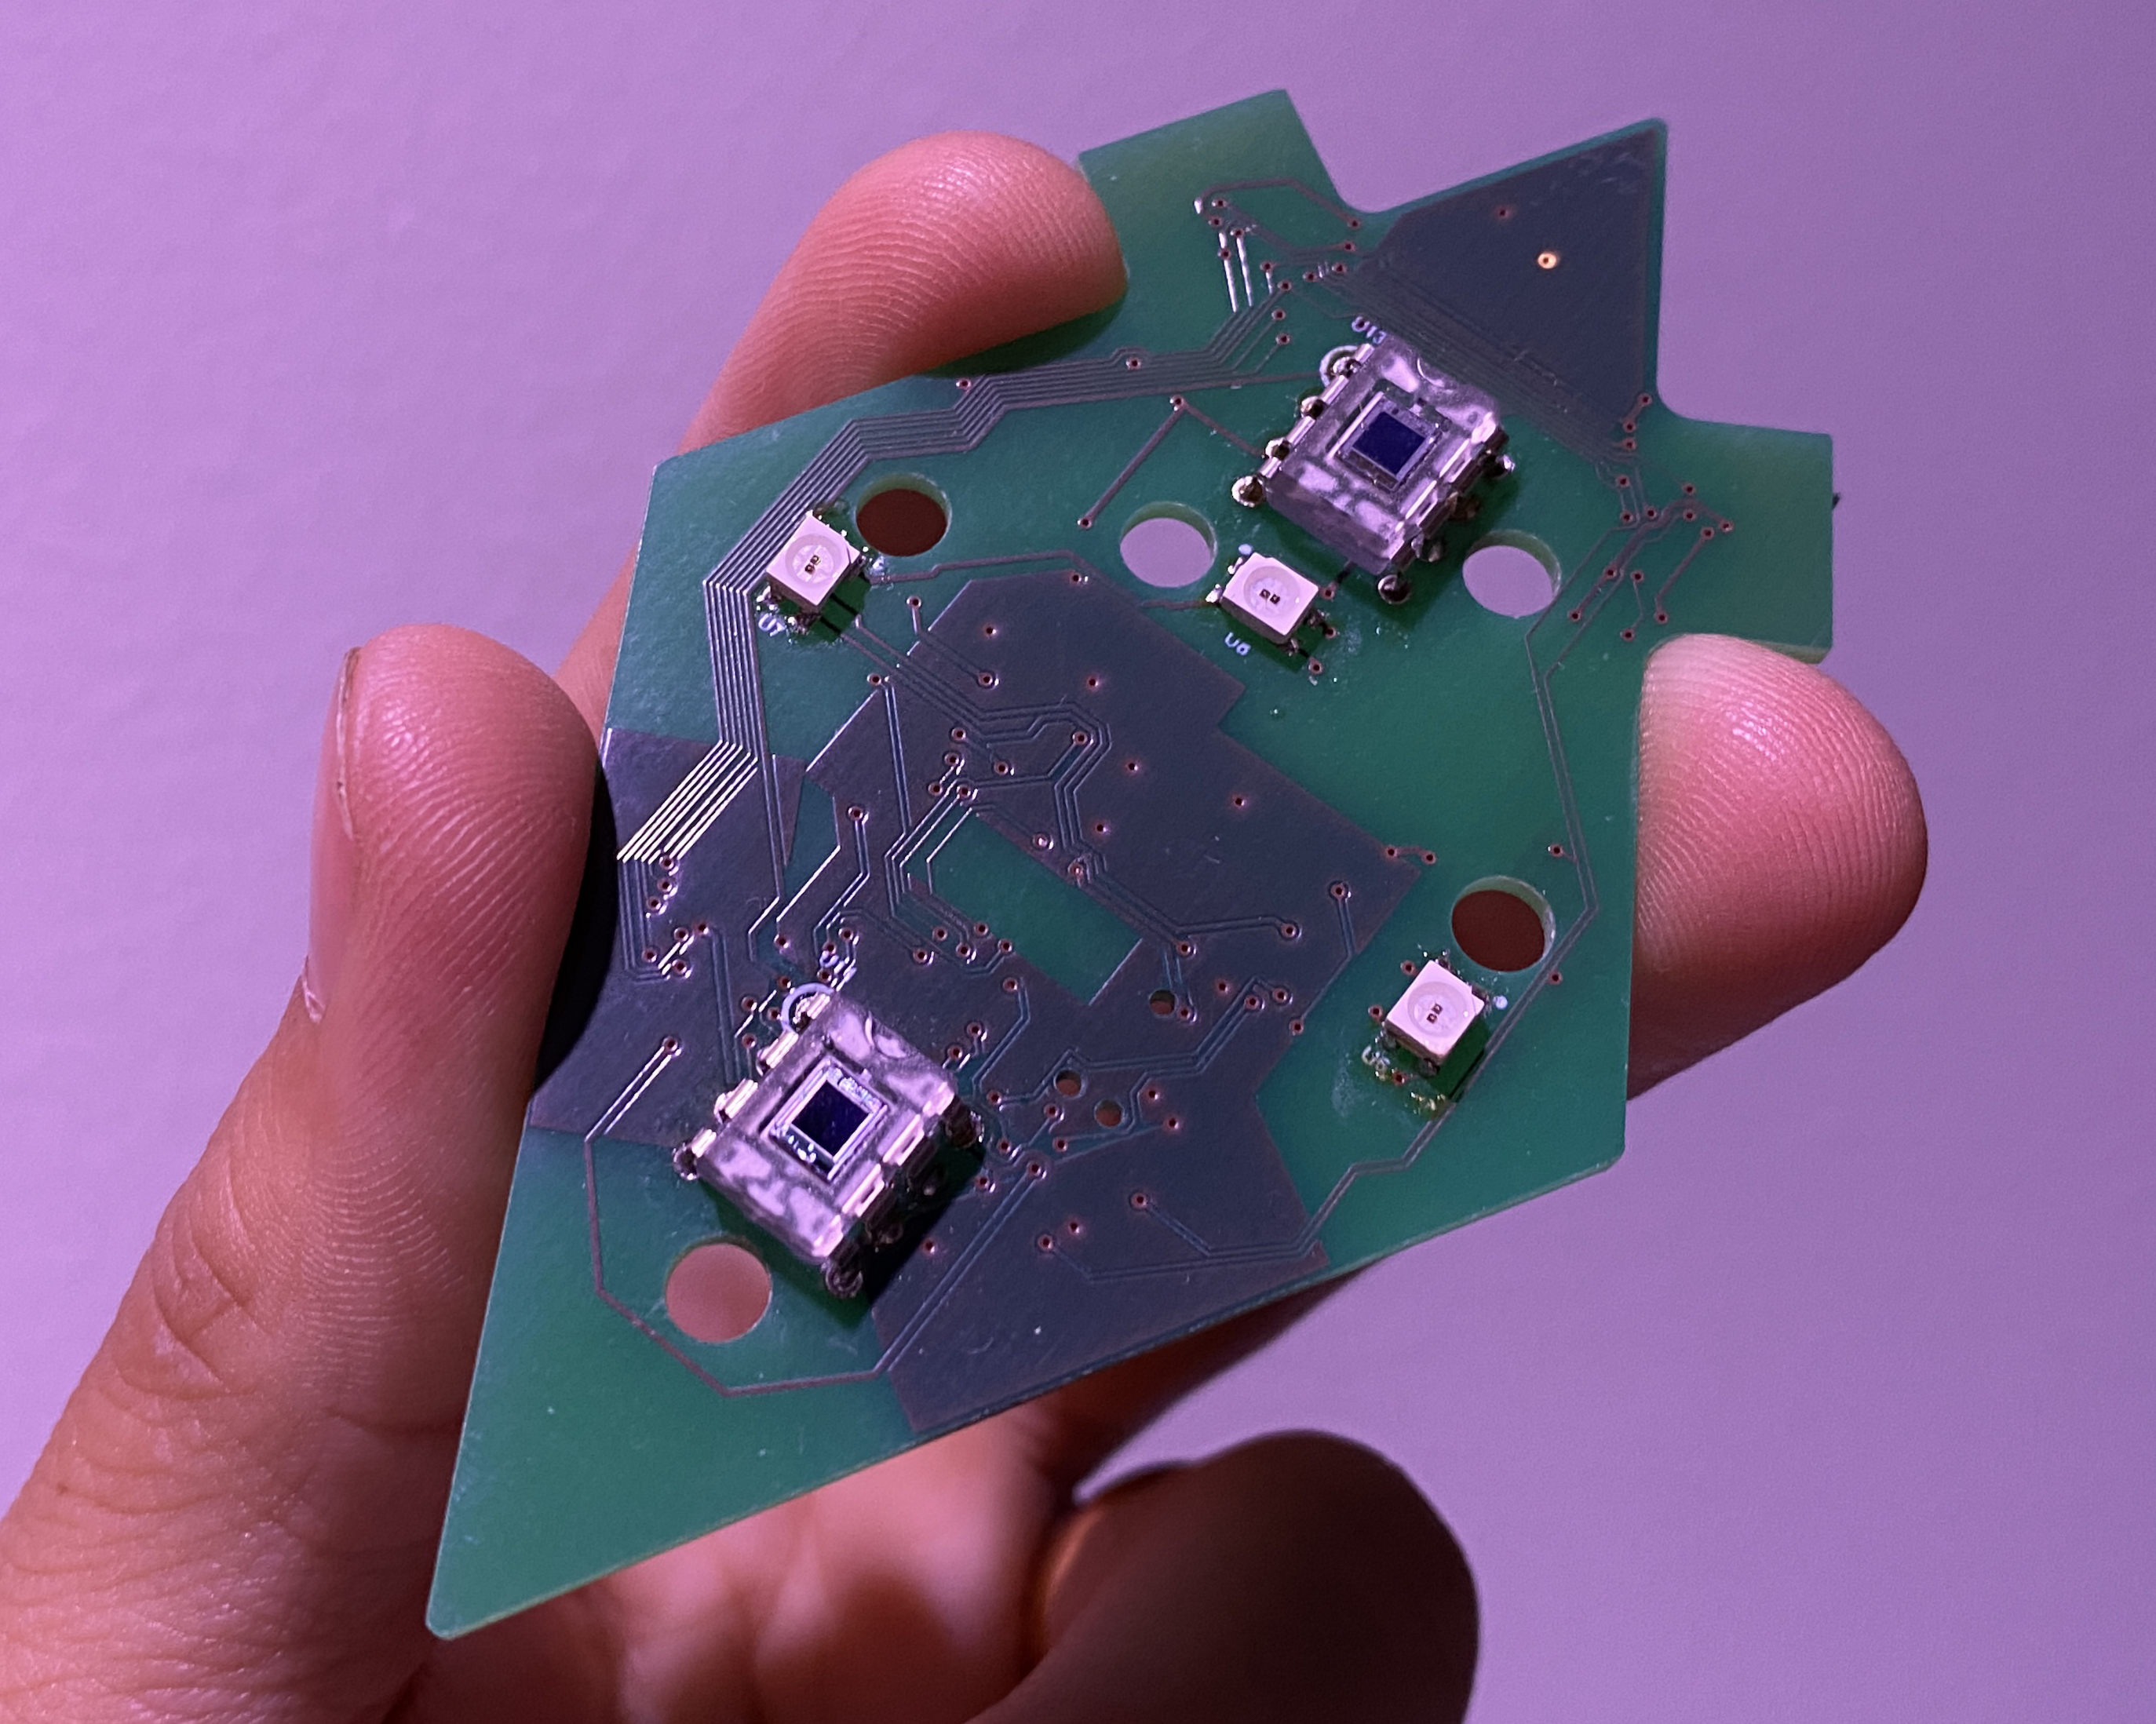
\includegraphics[width=.3\textwidth]{fig/mobi/rigid_coupling.png}}
        \subfigure[]{\label{fig:rigidboxplot}\includegraphics[width=.3\textwidth]{fig/mobi/rigidboxplot.pdf}}
        \subfigure[]{\label{fig:rigidcount}\includegraphics[width=.3\textwidth]{fig/mobi/rigidcount.pdf}}
        \subfigure[]{\label{fig:flex_coupling}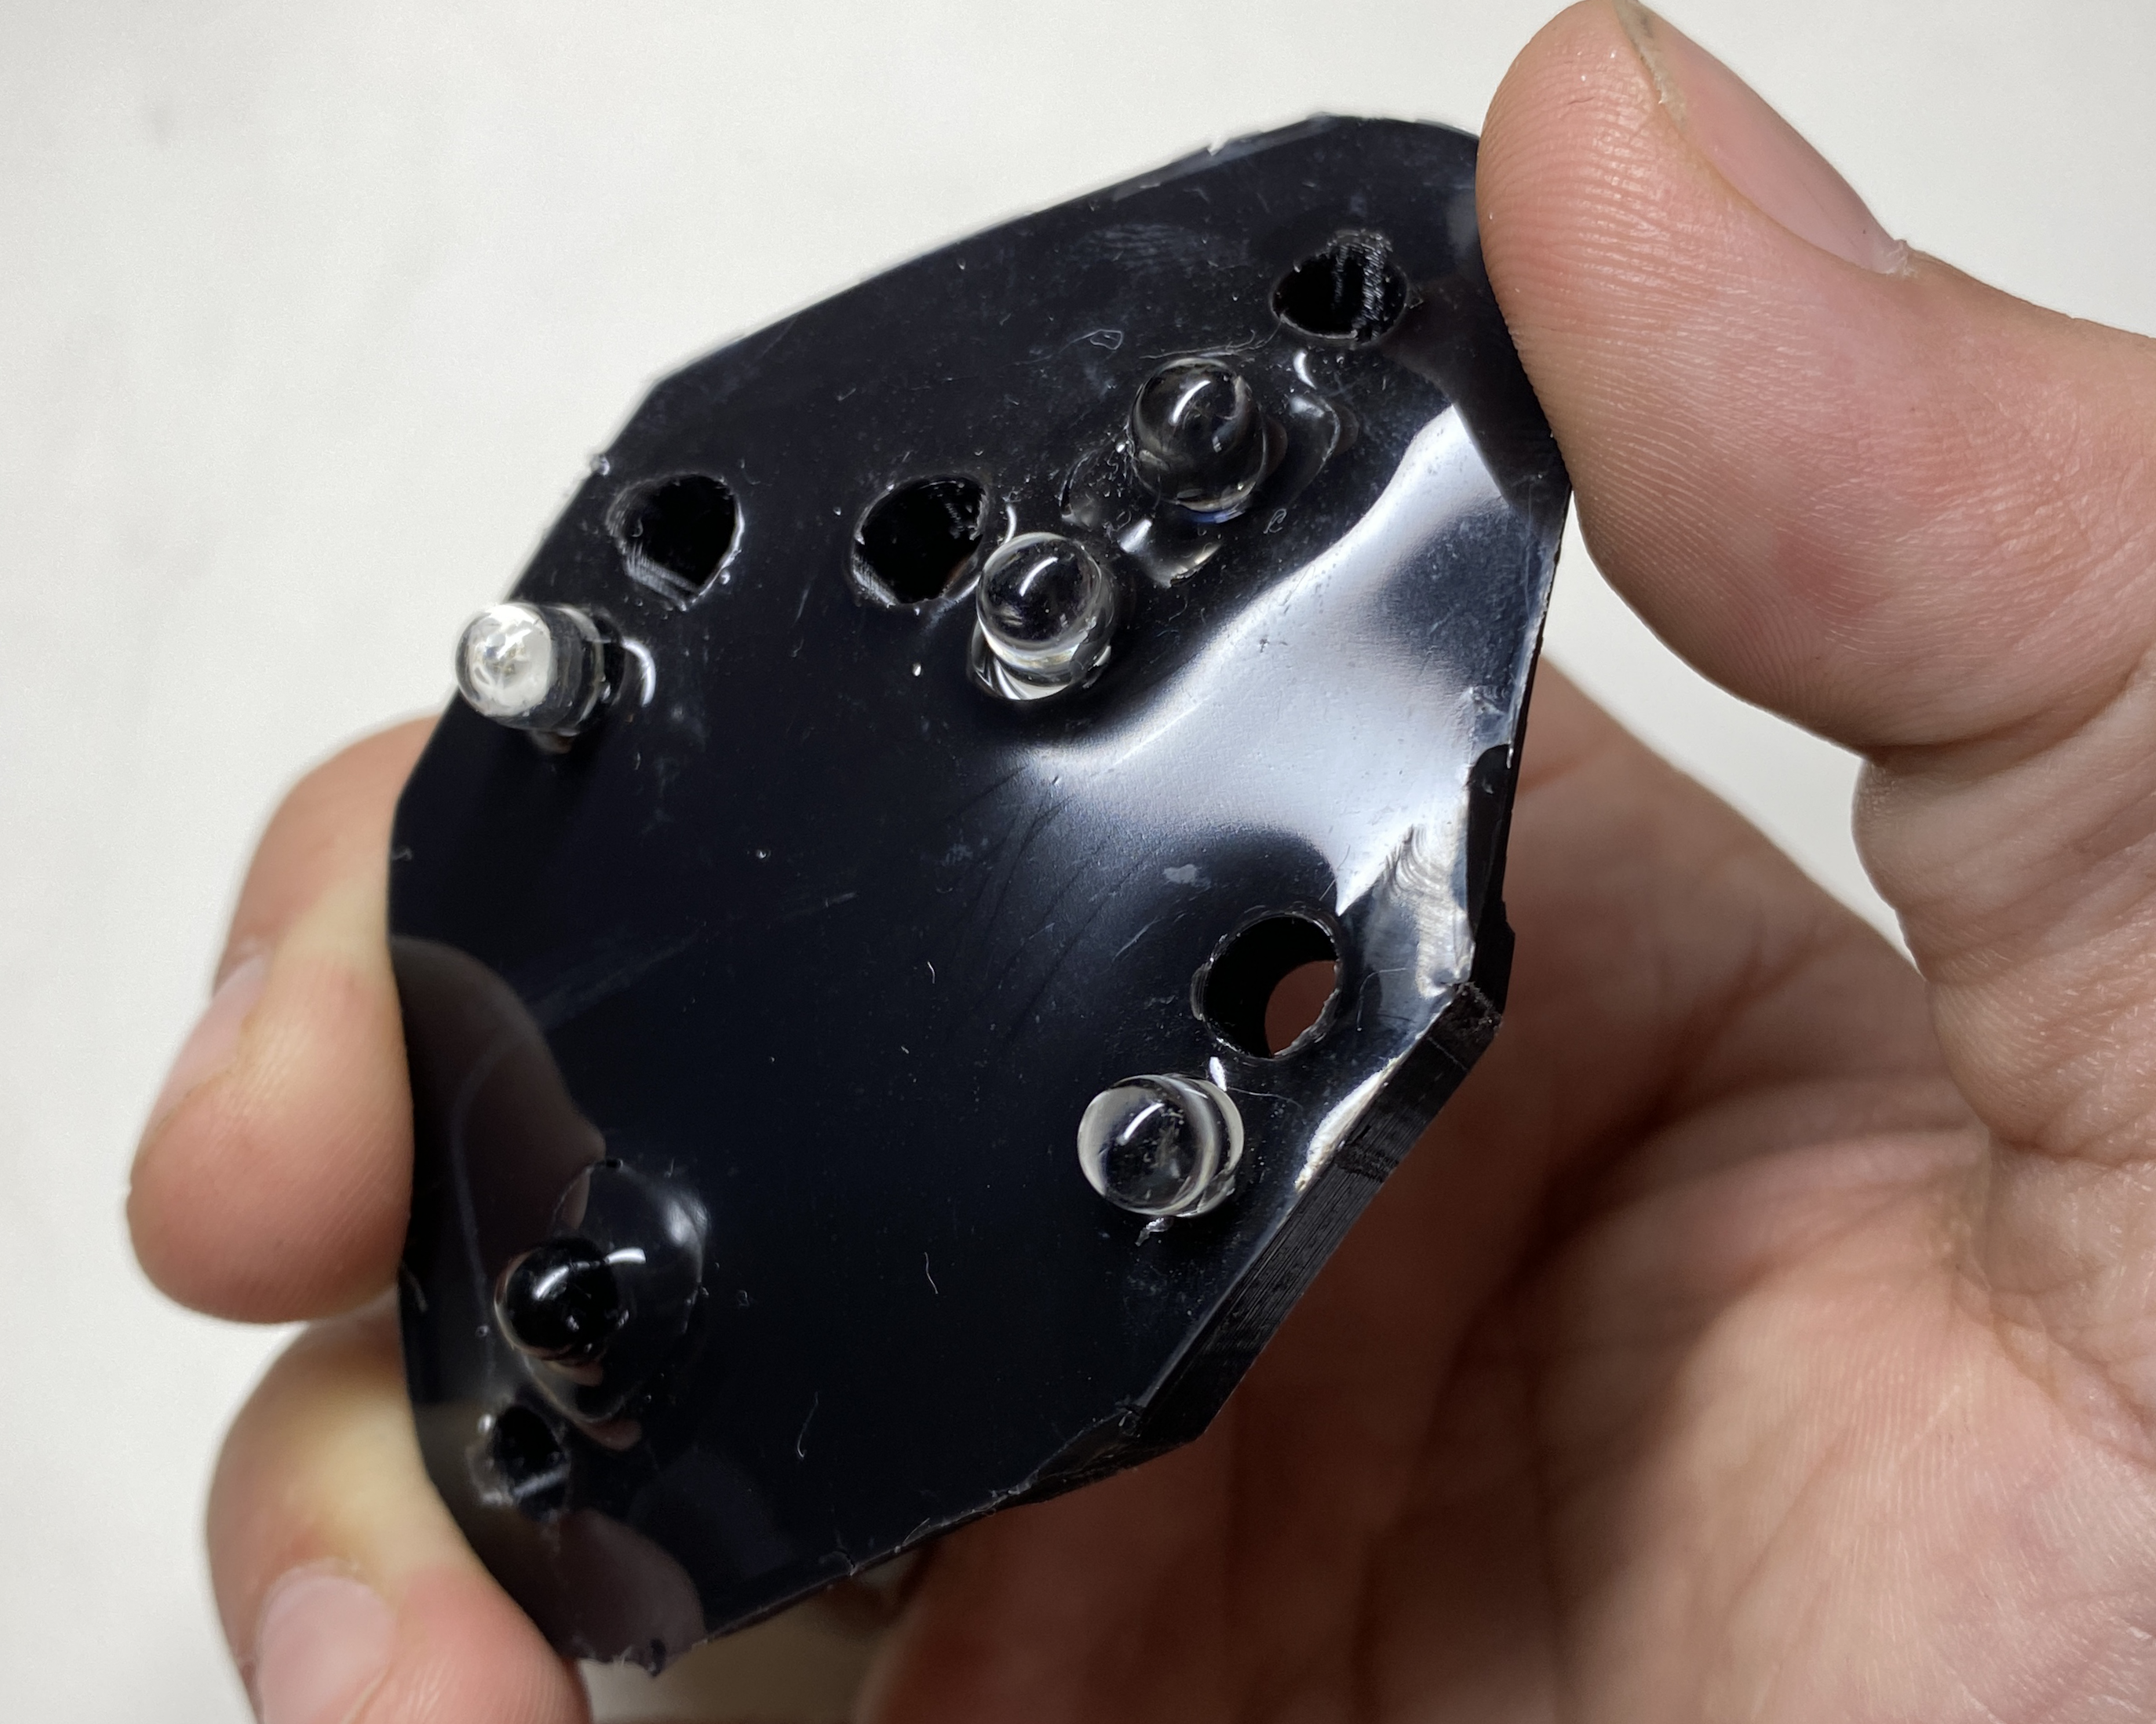
\includegraphics[width=.3\textwidth]{fig/mobi/flex_coupling.png}}
        \subfigure[]{\label{fig:flexibleboxplot}\includegraphics[width=.3\textwidth]{fig/mobi/flexibleboxplot.pdf}}
        \subfigure[]{\label{fig:flexiblecount}\includegraphics[width=.3\textwidth]{fig/mobi/flexiblecount.pdf}}
	\end{center}
	\caption{(a) A rigid-based board showing three sources and two detectors. (b) Boxplot showing the distance from optode locations to the center of the sphere using rigid modules. The red line denotes the average distance of all 25 optodes. The dashed green line represents the expected distance to the center given the 5~mm thickness of the modules. (c) A histogram of the distances reveals that the rigid-based probe does not conform to the sphere, leading to optodes being farther away from the surface, especially those optodes closer to the edge of the module. (d) A flexible-circuit-based board showing three sources and two detectors with light guides. (e) Boxplot showing the distance from the optodes to the center of the sphere of the flexible-circuit-based probe. (f) The histogram of the flexible-circuit-based probe optode distances.} 
	\label{fig:coupling}
\end{figure} 
A 5-module probe, in a configuration identical to layout 2 in Fig.~\ref{fig:layout2}, was placed on a 100~mm radius sphere. The 25 optodes were digitized using a hand-held Polhemus digitizer and the distance to the center of the sphere was calculated for each optode in both probes (Figure~\ref{fig:coupling}). The digitization was conducted on both flexible-circuit-based and rigid-based modules [Figs.~\ref{fig:rigid_coupling} and ~\ref{fig:flex_coupling}]. 

Fig.~\ref{fig:rigidboxplot} shows the average distance to the center of the sphere for all optodes of a rigid-board-based probe to be 107.5~mm with a range of 10.5~mm. In contrast, the average distance to the center decreases to 104.9~mm with flexible-circuit-based boards that allow the module to conform to the spherical surface [Fig.~\ref{fig:flexibleboxplot}]. Additionally, the range of distances decreases when using flexible-circuit-based modules. Fig.~\ref{fig:rigidcount} reveals a skewed left histogram, indicating that optodes near the edges of rigid modules remain farther from the scalp. Fig.~\ref{fig:flexiblecount}, however, shows that by using flexible-circuit-based modules, the same optode layout within a module results in optode distance closer to the scalp, indicating the ability of flexible-circuit-based modules to conform to the surface. 


\subsection{Automatic optode positioning}
\begin{figure}
	\begin{center}
    %\includegraphics[width=.3\textwidth]{fig/mobi/dig_pol4.png}
        \subfigure[]{\label{fig:domesetup}\includegraphics[width=.3\textwidth]{fig/mobi/domesetup.pdf}}
        \subfigure[]{\label{fig:digit3d}\includegraphics[width=.4\textwidth]{fig/mobi/digit3d.pdf}}
        \subfigure[]{\label{fig:digit1module}\includegraphics[width=.35\textwidth]{fig/mobi/digit1module.pdf}}
        \subfigure[]{\label{fig:digitpermodule}\includegraphics[width=.35\textwidth]{fig/mobi/digitpermodule.pdf}}
	\end{center}
	\caption{(a) Flexible-circuit-based Modular Optical Brain Imager (MOBI) modules arranged in probe layout 2 (from Figure~\ref{fig:layouts}) on top of a 100~mm radius sphere. (b) Spline model between 5 MOBI modules (green line) from which source (red crosses) and detector (blue crosses) positions are derived. Automatic optode digitization overlaid on manual digitization results (cyan circles). (c) Digitization error distribution averaged over all five modules in the probe. A green asterisk indicates the average digitization error. (d) Digitization errors are grouped by module.} 
	\label{fig:digitization}
\end{figure} 
Fig.~\ref{fig:digit3d} shows the traditional hand-held-based optode locations against the resulting optode locations using internal orientation sensors. For visibility, the optode locations are displayed over a 100~mm radius sphere. The cyan circles are optode locations averaged across five repetitions of hand-held digitizations. The standard deviation across those five hand-held digitizations was 1.78~mm. Fig.~\ref{fig:digit1module} shows the average digitization error over all optodes, defined as the Euclidian distance between the orientation-sensor-based location and the hand-held-based location. The average orientation-based error was 1.4~mm. Fig.~\ref{fig:digitpermodule} shows the same digitization error with optodes grouped by module. For all five modules, the average digitization error was less than 2~mm.  


\subsection{Cuff occlusion results}
% add results from Artinis as well for easy comparison. Side to side with MOBI results
\begin{figure}
	\begin{center}
    %\includegraphics[width=.49\textwidth]{fig/mobi/cuffmobi.pdf}
	   \subfigure[]{\label{fig:cuffmobi}\includegraphics[width=.49\textwidth]{fig/mobi/cuffmobi.pdf}}
	   \subfigure[]{\label{fig:cuffartinis}\includegraphics[width=.49\textwidth]{fig/mobi/cuffartinis.pdf}}
	\end{center}
	\caption{Results from a dual-pressure blood occlusion experiment using (a) a single Modular Optical Brain Imager module and (b) a single Artinis channel placed on the forearm. Venous (100~mmHg) and arterial (220~mmHg) occlusions lasted 75 seconds each prior to release. Oxygenated, deoxygenated, and total hemoglobin concentrations are shows in red, blue, and green lines, respectively.} 
	\label{fig:cuff}
\end{figure} 
Fig.~\ref{fig:cuff} shows the resulting changes in hemoglobin concentrations during the dual-pressure blood cuff occlusion experiment. During venous occlusion, both oxygenated (HbO) and deoxygenated (HbR) hemoglobin increase for both systems [Figs.~\ref{fig:cuffmobi} and \ref{fig:cuffartinis}]. The arterial occlusion resulted in a negative correlation between HbO and HbR, as demonstrated by the horizontal HbT line. Additionally, the \ac{MOBI} module captured the hyperemic peak typically observed when occlusion is suddenly released. 


\subsection{Finger-tapping results}
%Comment width/std for each of the hrf functions - "the lighter-colored, shaded areas depict standard error across trials"
%add probe plot with 5 channels. 
%Add second plot with module overlaid on atlas
\begin{figure}
	\begin{center}
	\includegraphics[width=0.6\textwidth]{fig/mobi/hrf.pdf}
	\end{center}
	\caption{Block average results from a finger-tapping experiment with a Modular Optical Brain Imager module placed over the left motor cortex centered on C3 in the standard 10-20 system. Solid lines are oxygenated and dashed lines are deoxygenated hemoglobin. Magenta, cyan, and orange lines represent different channels within the probe.}
	\label{fig:hrf}
\end{figure} 
Fig.~\ref{fig:hrf} shows the resulting hemodynamic response function (HRF) after block-averaging during a finger-tapping experiment. The stimulus lasted 10 seconds with a 20-second break in between, repeated 10 times. A clear hemodynamic response is shown with an increase in HbO of 60~uM approximately 10 seconds after stimulus onset. All channels demonstrated the expected increase in HbO and decrease in HbR, albeit channels over the motor cortex show a larger amplitude response. 



%%%% DISCUSSION %%%%
\section{Discussion}
\label{chap:mobi:discussion}
While many modular \ac{fNIRS} systems have brought about advantages such as portability, scalability, and modularity, to our knowledge this is the first 3-D aware and fully flexible-circuit-based system. \ac{MOBI}'s features are especially important for transitioning \ac{fNIRS} from laboratory/clinical settings to natural environments. With the expected higher physical movements in these new settings, we must find new and simpler methods to ensure optode-to-scalp coupling during use. Additionally, for true wearable commercial adoption, the \ac{fNIRS} community needs to rely less on expensive and cumbersome technology, such as 3-D tracking systems, for system setup. \ac{MOBI}'s automatic connection topology detection and IMU-based optode positioning do just that\textemdash they provide the necessary technical quantification for highly accurate 3-D modeling without the need for lots of user input and knowledge, enabling not only a wearable system but a usable one too. 

%% System characterization
Additionally, the system's usability is improved without affecting its performance. Fig.~\ref{fig:snr} shows \ac{MOBI}'s large dynamic range, an important consideration for modular, full-head systems with multiple channels of various SD separations. A high SNR is achieved for large SD separation while keeping safety considerations in mind. For example, the holes designed into the modules used for clearing hair also provide cooling. The double-sided board design places only optodes on the scalp-facing side, limiting all driving electronics to the non-contact side, allowing for further heat dissipation for long-term wear. With a measured 9.8~m$\Omega$ resistance for each module, 75 modules can be theoretically connected prior to the 5~V supply power dropping below the necessary 3.3~V to drive the microcontrollers, far above the approximate 20 modules needed for a full head probe. Excluding the master board and any fabric to further block light, a full-head 20-module probe would weigh 280~grams (about the weight of an average bicycle helmet)\textemdash lightweight enough for long-term wear. %Compare that to the weight of a helmet. -> 14 gram * 20 = 280 grams. high-end bike helmets = 190. Average around 380 grams.  

%% Spatial multiplexing improvement
Full-head modular probes not only require lightweight modules and large dynamic ranges but also an encoding strategy to ensure fast full frame rates. Fig.~\ref{fig:layouts} shows how a spatial multiplexing encoding strategy can improve a full probe's sampling rate by leveraging a probe's layout rather than the total number of sources. As long as sources are spatially dispersed based on their performance, contributions to a detector's readings avoid cross-talk. As the probes become denser and the number of channels increases (Table~\ref{tab:layouts}, Row 3), the distance between sources decreases, and the number of SMGs must increase to prevent cross-talk. Similarly, as 2-D probes are placed on 3-D surfaces, the Euclidean distance between sources decreases, which may require further SMG refinement. Although spatial multiplexing can be easily implemented and doesn't require extensive hardware, it does require knowledge of the location of all sources and detectors to identify the SMGs for a particular probe\textemdash a functionality that many systems currently do not possess without the use of external digitization tools.  

%% Source-scalp coupling
In addition to increasing the full frame rate of a probe, modular \ac{fNIRS} systems must ensure proper source-to-scalp coupling during high-movement use in natural settings. Fig.~\ref{fig:coupling} compares a rigid board and a flexible-circuit-based board's ability to conform to a surface. Rigid modules have minimal direct contact with the scalp and rely on mechanical/protruding couplers on the optodes or curved board designs tailored toward specific head shapes. Fig.~\ref{fig:coupling} highlights the source-to-scalp gaps inherent in rigid-board designs. Therefore, designers of rigid boards must balance between designing smaller boards to increase source-scalp coupling or designing larger boards that allow for larger SD separations. Our flexible-circuit-based boards allow for both. 

%% Automatic optode positions
Finally, not only is source-to-scalp coupling important, but an \ac{fNIRS} system must also constantly measure the position of each optode during use. Fig.~\ref{fig:digitization} validates the accuracy of our internal IMU-based optode positioning system. It demonstrates that the average error between \ac{MOBI}'s IMU-based optode digitization and the traditional Polhemus-based digitization is only 1.4~mm. The positioning error is less than the variability of repeated handheld-based digitization systems. This method requires knowledge of the probes connection topology, assumes fixed FPC cable lengths, and requires knowledge of the module geometry and optode layout. Although automatic optode digitization can drastically reduce the time it takes to set up \ac{fNIRS} systems, it does require appropriate hardware support such as a \ac{P2P} network and orientation sensors on each module. Although we have seen the use of orientation sensors in modular systems for motion artifact correction, to our knowledge, this is the first use of IMU for internal-based optode positioning and decreasing system setup times.

%% Cuff occlusion and finger tapping results
Fig.~\ref{fig:cuff} shows the results of validating our \ac{MOBI} system against a commercial \ac{fNIRS} system. As expected, both systems show an increase in both HbO and HbR during venous occlusion. When the pressure increases above systolic pressure, we see a negative correlation between HbO and HbR due to the muscles depleting blood oxygen during the occlusion of arterial blood. Finally, the hyperemia peak seen at 180~seconds corresponds to the increase in blood flow that occurs following arterial occlusion. Not only do both systems capture the same physiological traces, but the traces are consistent with previous research results~\cite{Liu2022}. Similarly, Fig.~\ref{fig:hrf} shows the results of a finger-tapping experiment. As expected, the HRF shows an increase in HbO and a decrease in HbR during a task that utilizes the motor cortex. Although we cannot say anything about our system's performance across a population due to it being a study of N=1, these experiments demonstrate that \ac{MOBI}'s ability to extract tissue hemodynamics and brain activity is comparable to existing commercial systems. 

%% Limitations
Our \ac{MOBI} system has limitations despite directly addressing many usability concerns of wearable systems. First, spline models onto which optode layouts are superimposed rely on the assumption that the distance between modules is fixed. In \ac{MOBI}, we use 14~mm length non-stretchable FPC cables that provide a 2~mm gap between modules once connected to the FPC connector. As \ac{MOBI} samples neighboring IMUs, it fixes the spline distance between modules. Depending on the cap design, this assumption may not hold true for other \ac{fNIRS} systems (for example, if modules are placed on stretchable fabric). Second, while connecting modules using FPC cables assists with determining the connection topology, it makes it difficult to remove a single module from a dense probe to adjust hair under a particular region. Rather, our \ac{MOBI} system uses two caps\textemdash a sparse mesh cap that holds the probe in place while a user uses the holes to access and adjust hair under optodes, and a second cap placed after hair adjustment to further block stray light. Third, the finger-tapping results were conducted on a subject with short hair. Further investigations into the effect of hair artifacts on signal quality must be performed. Finally, although \ac{MOBI} data can be saved in the standardized SNIRF format, our data acquisition Processing-based GUI requires users to learn and work in a new interface. Future work includes integrating our work with the open-source middleware Lab Streaming Layer~\cite{LSL2014} for easier synchronization and recording of \ac{fNIRS} and auxiliary data. 


% --- EOF ---